\chapter{Experimental Evaluation}\label{experiment}

\section{Flocking in Free Sapce}

\subsection{Comparison with Flocking model}

we first simulate the flocking model with various $a_{ij}$ and control laws in Chapter~\ref{flocking} with 2, 3 and 4 agents respectively. The initial position are illustrated in Figure~\ref{fig:simulate_flocking} where only the most front agent has initial velocity pointing forward.
\begin{figure}[htb]
	\centering
	\subfigure[Two agents in a shape of straight line]{\label{fig:2_agents}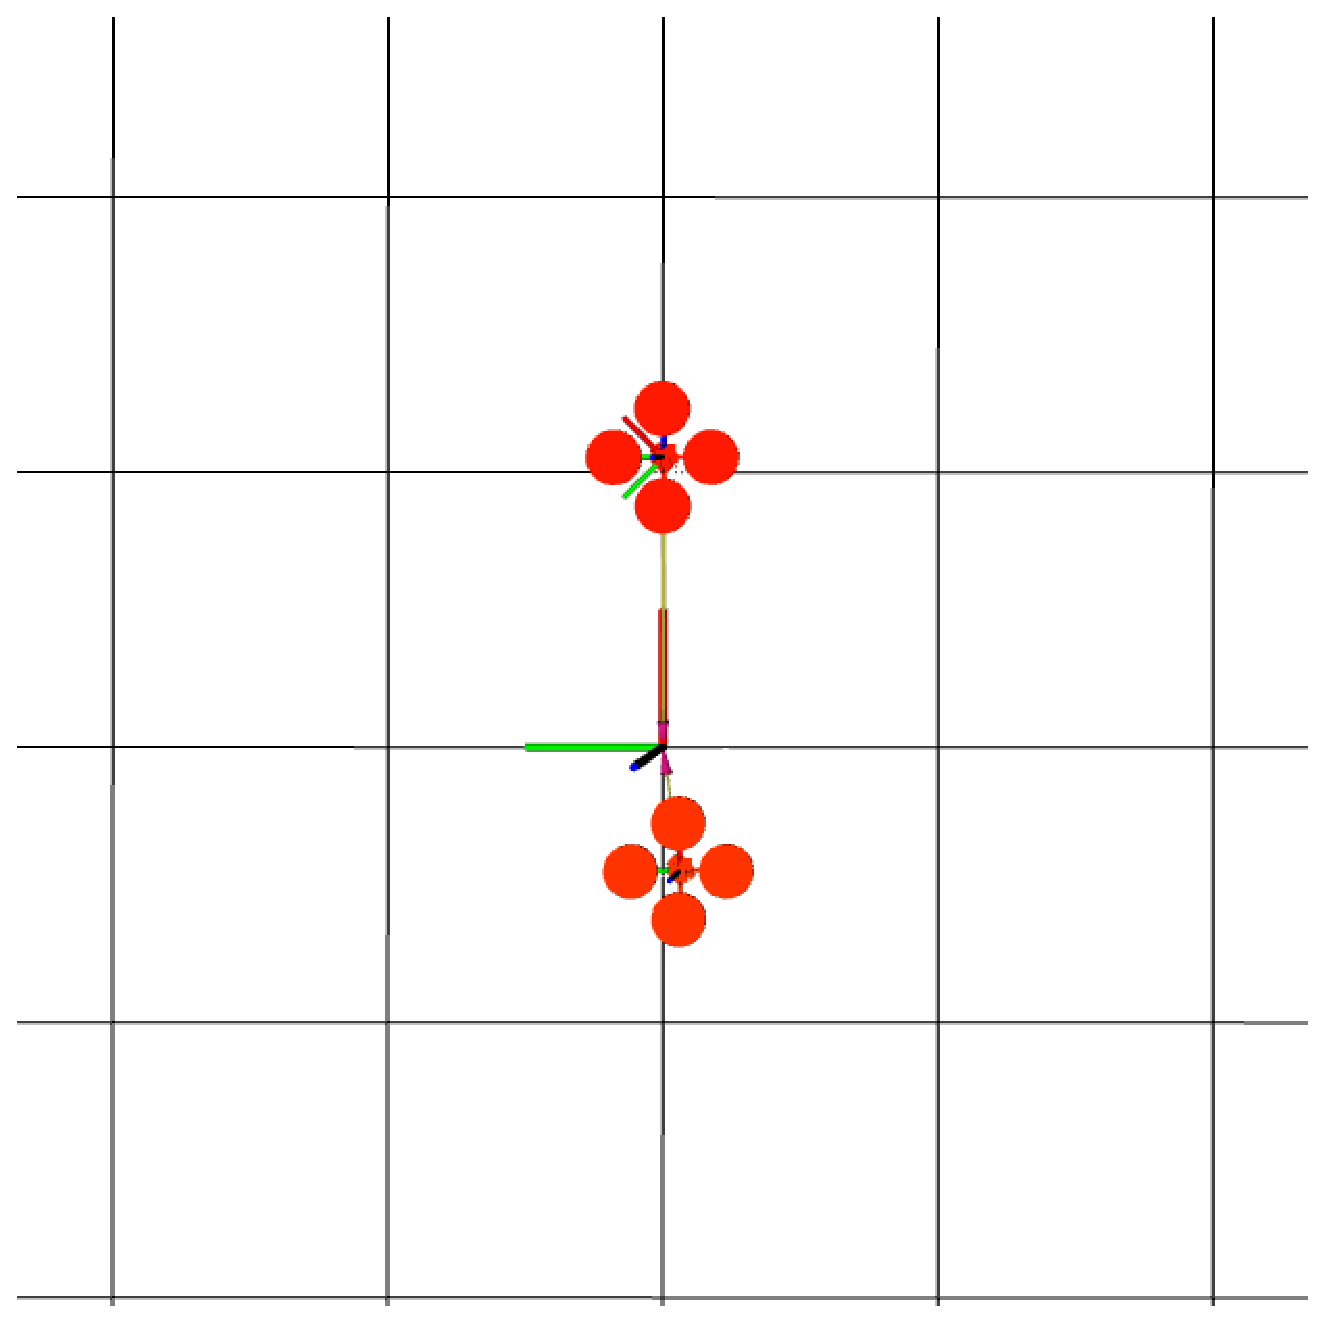
\includegraphics[width=0.32\textwidth]{figure/2_agents.eps}}
	\subfigure[Three agents in a shape of equilateral triangle]{\label{fig:2_agents}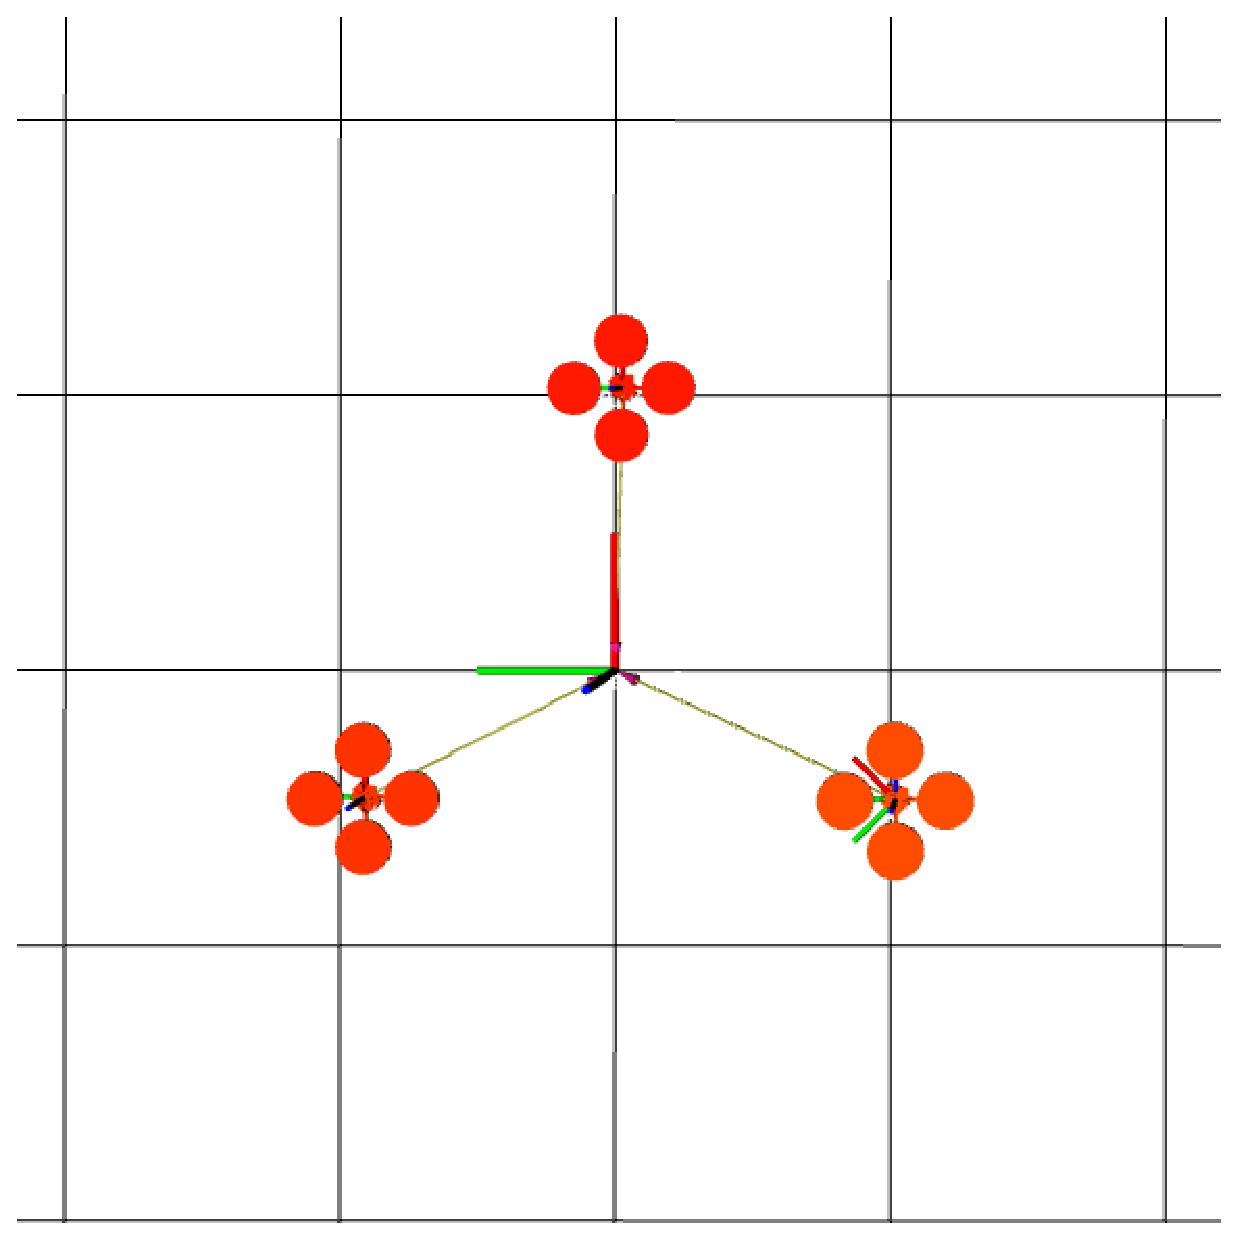
\includegraphics[width=0.31\textwidth]{figure/3_agents.eps}}
	\subfigure[Four agents in a shape of diamond]{\label{fig:2_agents}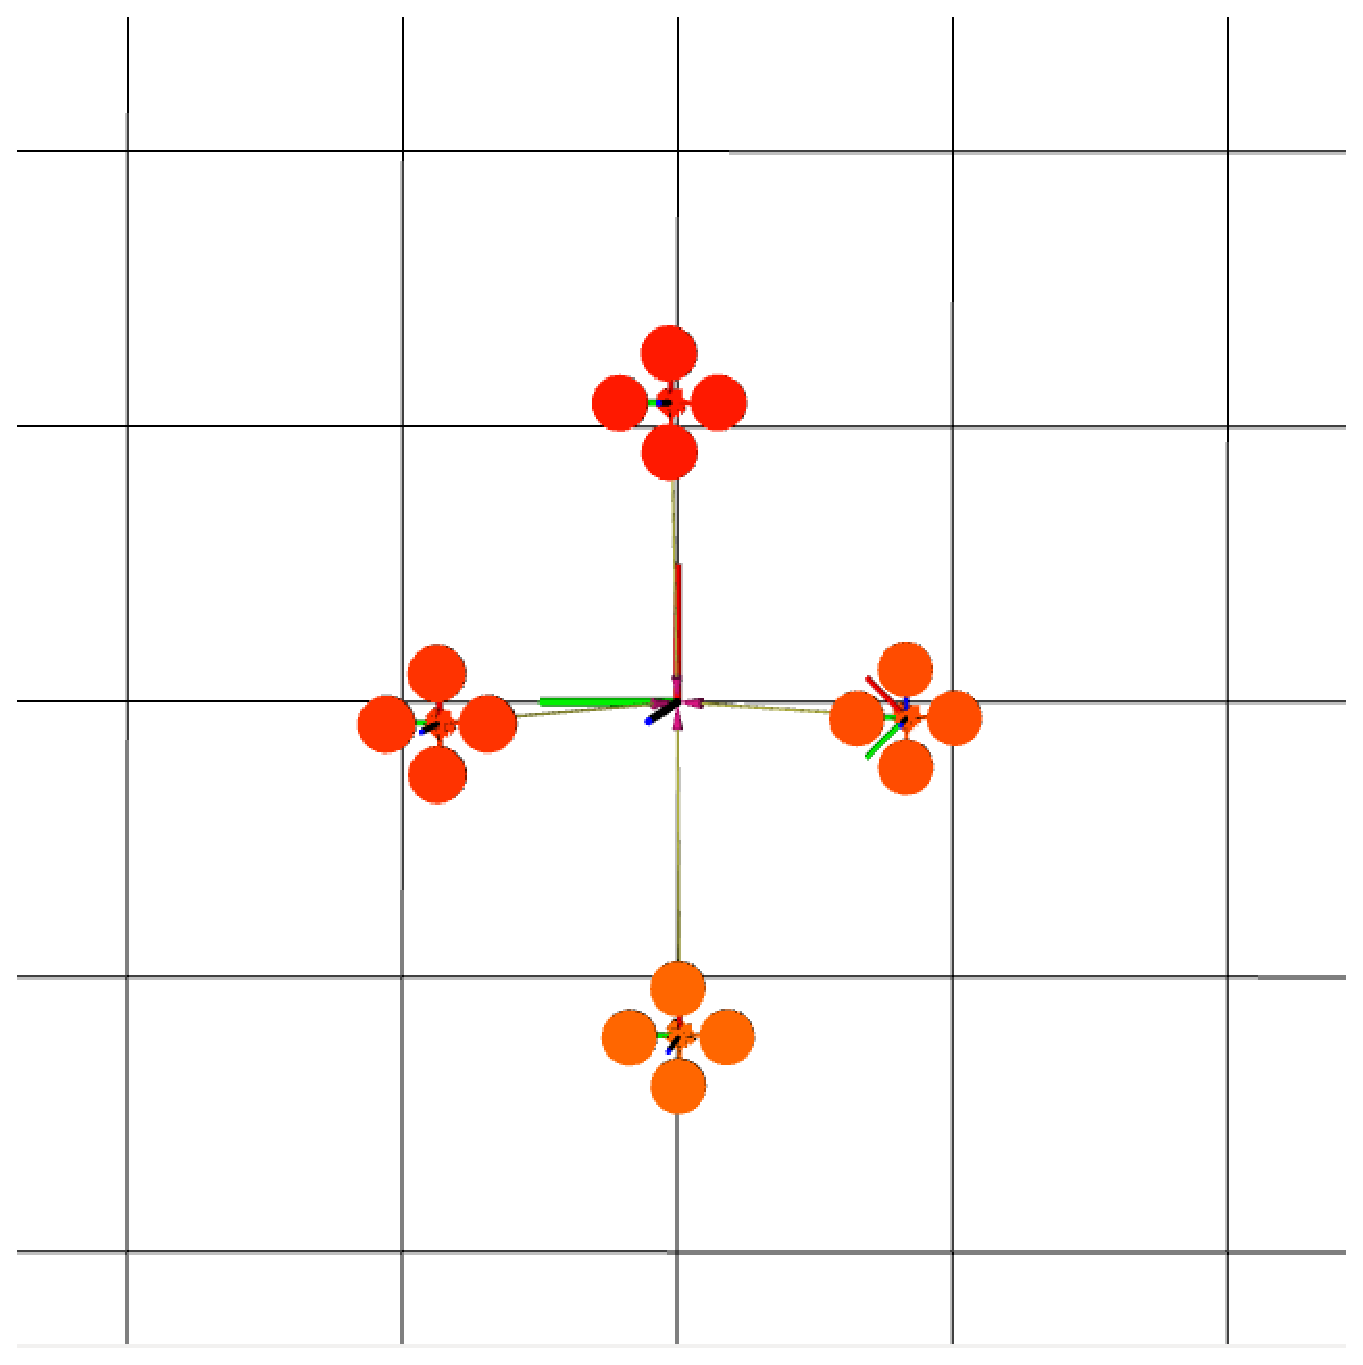
\includegraphics[width=0.33\textwidth]{figure/4_agents.eps}}
	\caption{Simulations of multi-UAV flocking}\label{fig:simulate_flocking}
\end{figure}

\section{Flocking in Cluttered Environment}